% !TEX TS-program = pdflatex
\documentclass[11pt]{article}
\usepackage[a4paper,margin=1in]{geometry}
\usepackage{amsmath,amssymb,amsthm}
\usepackage{mathtools}
\usepackage{bm}
\usepackage{enumitem}
\usepackage{graphicx}
\usepackage{tikz}
\usepackage{pgfplots}
%\pgfplotsset{compat=1.18}
\usetikzlibrary{arrows.meta,calc,positioning,shapes,patterns}
\usepackage[colorlinks=true,linkcolor=blue,citecolor=blue,urlcolor=blue]{hyperref}
\usepackage{microtype}

% Theorem-style environments
\newtheorem{definition}{Definition}
\newtheorem{theorem}{Theorem}
\newtheorem{proposition}{Proposition}
\newtheorem{example}{Example}
\newtheorem{remark}{Remark}

% Custom commands
\newcommand{\N}{\mathbb{N}}
\newcommand{\Z}{\mathbb{Z}}
\newcommand{\Q}{\mathbb{Q}}
\newcommand{\R}{\mathbb{R}}
\newcommand{\C}{\mathbb{C}}
\newcommand{\powerset}{\mathcal{P}}
\newcommand{\im}{\operatorname{im}}
\newcommand{\dom}{\operatorname{dom}}
\newcommand{\codom}{\operatorname{codom}}
\newcommand{\id}{\mathrm{id}}

\title{Lecture: Sets and Functions}
\author{\vspace{-0.5em}Mathematical Economics — Core Tools}
\date{\vspace{-0.5em}\today}

\begin{document}
\maketitle
\tableofcontents
\bigskip

\section{Sets}
\begin{definition}[Set]
A \emph{set} is a collection of distinct objects, called elements. If $x$ is an element of a set $A$, we write $x\in A$; otherwise $x\notin A$.
\end{definition}

\subsection{Describing Sets}
\begin{itemize}[leftmargin=*]
  \item \textbf{Roster notation:} $A=\{1,2,3\}$. 
  \item \textbf{Set-builder notation:} $B=\{x\in \Z: x\text{ is even}\} = 2\Z$. 
  \item \textbf{Intervals in $\R$:} $(a,b)$, $[a,b]$, $(a,b]$, $[a,b)$.
\end{itemize}

\begin{example}
Let $S=\{(i,j)\in\Z^2: i+j=4\}$. Then $S=\{(0,4),(1,3),(2,2),(3,1),(4,0)\}$.
\end{example}

\subsection{Subsets and Equality}
\begin{definition}[Subset]
$A\subseteq B$ if every element of $A$ is in $B$. If $A\subseteq B$ and $B\subseteq A$, then $A=B$.
\end{definition}

\begin{proposition}[Basic Laws]
For any sets $A,B,C$ in a universe $U$:
\begin{enumerate}[label=\arabic*.]
  \item $A\cap B=B\cap A$ (commutativity),\; $A\cup B=B\cup A$.
  \item $A\cap (B\cup C)=(A\cap B)\cup(A\cap C)$ (distributivity), similarly for $\cup$ over $\cap$.
  \item $(A^c)^c=A$,\; $A\cup A^c=U$,\; $A\cap A^c=\varnothing$ (complements).
\end{enumerate}
\end{proposition}

\subsection{Operations with Venn Diagrams}
\begin{center}
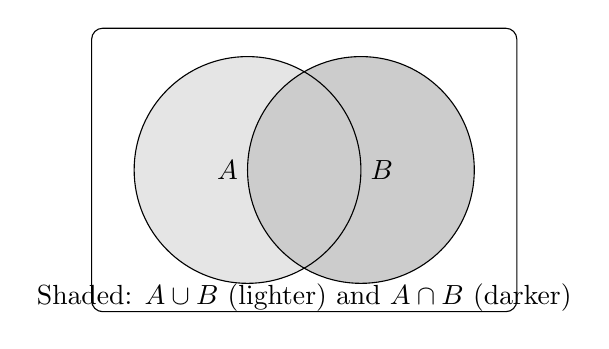
\begin{tikzpicture}[scale=0.9]
  % Universe rectangle
  \draw[rounded corners] (-3,-2) rectangle (3,2);
  % Sets
  \begin{scope}
    \clip (-3,-2) rectangle (3,2);
    \fill[gray!20] (-0.8,0) circle (1.6);
    \fill[gray!40] (0.8,0) circle (1.6);
  \end{scope}
  \draw (-0.8,0) circle (1.6) node[left] {$A$};
  \draw (0.8,0) circle (1.6) node[right] {$B$};
  \node at (0,-1.8) {Shaded: $A\cup B$ (lighter) and $A\cap B$ (darker)};
\end{tikzpicture}
\end{center}

\subsection{Power Set and Cartesian Product}
\begin{definition}[Power set]
The \emph{power set} of $A$ is $\powerset(A)=\{B: B\subseteq A\}$.
\end{definition}
\begin{example}
If $A=\{a,b\}$ then $\powerset(A)=\{\varnothing,\{a\},\{b\},\{a,b\}\}$.
\end{example}
\begin{definition}[Cartesian product]
$A\times B=\{(a,b): a\in A,\ b\in B\}$.
\end{definition}

\section{Relations and Functions}
\subsection{Relations}
A relation $R$ from $A$ to $B$ is a subset of $A\times B$. We write $a\,R\,b$ if $(a,b)\in R$.

\begin{example}
On $\Z$, the relation $\le$ is a subset of $\Z\times\Z$: $\le =\{(m,n): m\le n\}$.
\end{example}

\subsection{Functions}
\begin{definition}[Function]
A function $f$ from $A$ to $B$, written $f\colon A\to B$, assigns to each $a\in A$ a unique element $f(a)\in B$. Here $A$ is the \emph{domain} and $B$ a \emph{codomain}. The \emph{image} (range) is $\im(f)=\{f(a): a\in A\}\subseteq B$.
\end{definition}

\begin{center}
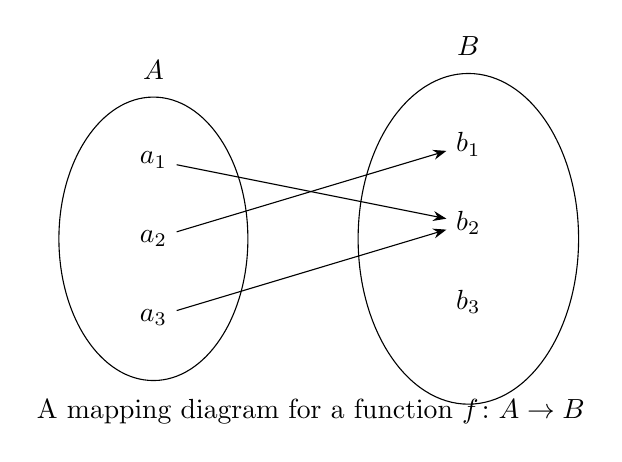
\begin{tikzpicture}[>=Stealth]
  % Two sets as ovals
  \draw (-2,0) ellipse (1.2 and 1.8) node[above=1.9cm] {$A$};
  \draw (2,0)  ellipse (1.4 and 2.1) node[above=2.2cm] {$B$};
  % Elements in A
  \node (a1) at (-2,1) {$a_1$};
  \node (a2) at (-2,0) {$a_2$};
  \node (a3) at (-2,-1) {$a_3$};
  % Elements in B
  \node (b1) at (2,1.2) {$b_1$};
  \node (b2) at (2,0.2) {$b_2$};
  \node (b3) at (2,-0.8) {$b_3$};
  % Arrows
  \draw[->] (a1) -- (b2);
  \draw[->] (a2) -- (b1);
  \draw[->] (a3) -- (b2);
  \node at (0,-2.2) {A mapping diagram for a function $f\colon A\to B$};
\end{tikzpicture}
\end{center}

\subsection{Images and Preimages}
For $S\subseteq A$, define $f[S]=\{f(a): a\in S\}\subseteq B$. For $T\subseteq B$, the preimage is $f^{-1}[T]=\{a\in A: f(a)\in T\}$.

\begin{example}
Let $f\colon \R\to\R$, $f(x)=x^2$. Then $f[(-2,1)]=[0,4)$ and $f^{-1}[(1,4]]=[-2,-1)\cup(1,2]$.
\end{example}

\subsection{Injective, Surjective, Bijective}
\begin{definition}
A function $f\colon A\to B$ is
\begin{itemize}[leftmargin=*]
  \item \emph{injective} (one-to-one) if $f(a)=f(a')\Rightarrow a=a'$;
  \item \emph{surjective} (onto) if $\im(f)=B$;
  \item \emph{bijective} if it is both injective and surjective.
\end{itemize}
\end{definition}

\begin{center}
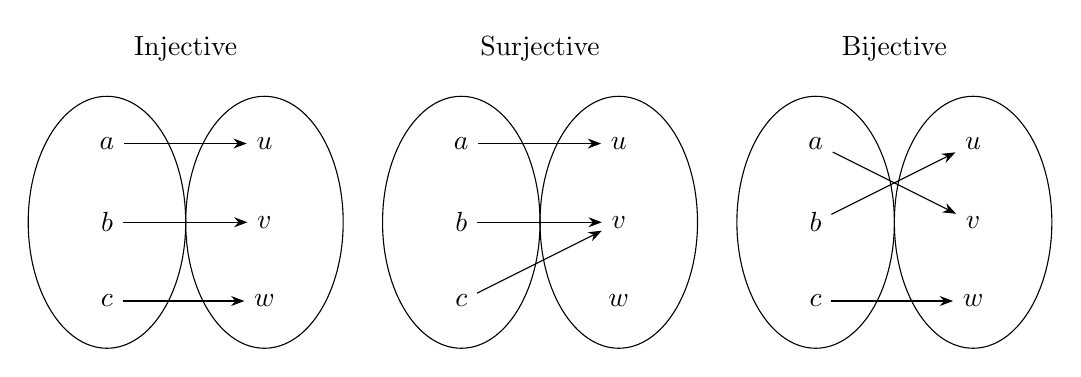
\begin{tikzpicture}[>=Stealth]
  \begin{scope}[xshift=-4.5cm]
    \node at (0,2.2) {Injective};
    \draw (-1,0) ellipse (1 and 1.6);
    \draw ( 1,0) ellipse (1 and 1.6);
    \foreach \y/\name in {1/a,0/b,-1/c} {\node (A\name) at (-1,\y) {$\name$};}
    \foreach \y/\name in {1/u,0/v,-1/w} {\node (B\name) at ( 1,\y) {$\name$};}
    \draw[->] (Aa) -- (Bu);
    \draw[->] (Ab) -- (Bv);
    \draw[->] (Ac) -- (Bw);
  \end{scope}
  \begin{scope}
    \node at (0,2.2) {Surjective};
    \draw (-1,0) ellipse (1 and 1.6);
    \draw ( 1,0) ellipse (1 and 1.6);
    \foreach \y/\name in {1/a,0/b,-1/c} {\node (A\name) at (-1,\y) {$\name$};}
    \foreach \y/\name in {1/u,0/v,-1/w} {\node (B\name) at ( 1,\y) {$\name$};}
    \draw[->] (Aa) -- (Bu);
    \draw[->] (Ab) -- (Bv);
    \draw[->] (Ac) -- (Bv);
  \end{scope}
  \begin{scope}[xshift=4.5cm]
    \node at (0,2.2) {Bijective};
    \draw (-1,0) ellipse (1 and 1.6);
    \draw ( 1,0) ellipse (1 and 1.6);
    \foreach \y/\name in {1/a,0/b,-1/c} {\node (A\name) at (-1,\y) {$\name$};}
    \foreach \y/\name in {1/u,0/v,-1/w} {\node (B\name) at ( 1,\y) {$\name$};}
    \draw[->] (Aa) -- (Bv);
    \draw[->] (Ab) -- (Bu);
    \draw[->] (Ac) -- (Bw);
  \end{scope}
\end{tikzpicture}
\end{center}

\subsection{Inverse and Composition}
\begin{definition}[Inverse]
If $f\colon A\to B$ is bijective, the \emph{inverse} $f^{-1}\colon B\to A$ satisfies $f^{-1}(f(a))=a$ and $f(f^{-1}(b))=b$.
\end{definition}
\begin{definition}[Composition]
If $f\colon A\to B$ and $g\colon B\to C$, then $(g\circ f)\colon A\to C$ is $(g\circ f)(a)=g(f(a))$.
\end{definition}

\begin{center}
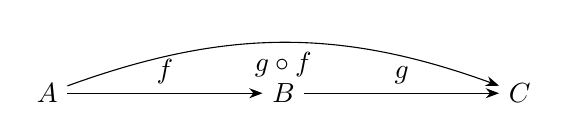
\begin{tikzpicture}[>=Stealth]
  \node (A) at (0,0) {$A$};
  \node (B) at (3,0) {$B$};
  \node (C) at (6,0) {$C$};
  \draw[->] (A) -- node[above] {$f$} (B);
  \draw[->] (B) -- node[above] {$g$} (C);
  \draw[->] (A) to[bend left=20] node[below] {$g\circ f$} (C);
\end{tikzpicture}
\end{center}

\subsection{Graphs of Real-Valued Functions}
A function $f\colon \R\to\R$ can be represented by its graph $\{(x,f(x)): x\in\R\}\subseteq\R^2$.

\begin{center}
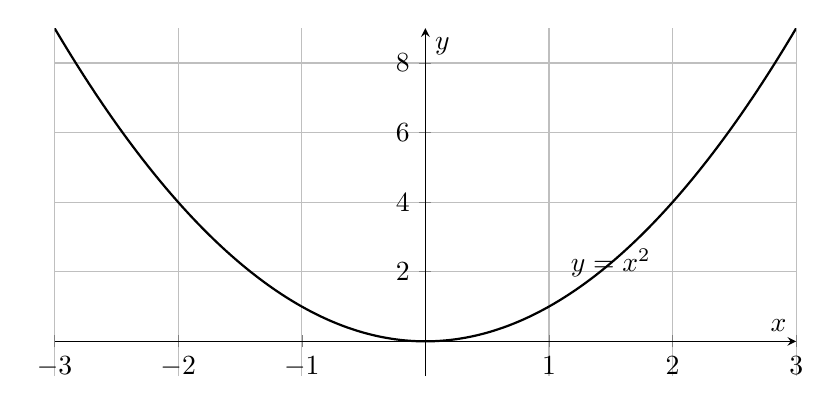
\begin{tikzpicture}
\begin{axis}[
  width=11cm,height=6cm,
  axis lines=middle,
  xlabel={$x$},ylabel={$y$},
  xmin=-3,xmax=3,ymin=-1,ymax=9,
  samples=200,domain=-3:3,
  grid=both
]
\addplot[thick] {x^2};
\node at (axis cs:1.5,2.25) {$y=x^2$};
\end{axis}
\end{tikzpicture}
\end{center}

\section{Worked Examples}
\begin{example}[Counting with Power Sets]
How many subsets does an $n$-element set have? \;\emph{Answer:} $|\powerset(A)|=2^n$, since each element can be either included or excluded.
\end{example}

\begin{example}[Injectivity and Surjectivity]
Consider $f\colon \Z\to\Z$, $f(n)=2n+1$. Then $f$ is injective (since $2n+1=2m+1\Rightarrow n=m$) but not surjective onto $\Z$ (even integers are not in the image).
\end{example}

\begin{example}[Images and Preimages]
Let $f\colon \R\to\R$, $f(x)=x^3$. For $S=[-1,2]$, we have $f[S]=[-1,8]$. For $T=[1,27]$, $f^{-1}[T]=[1,3]$.
\end{example}

\section{Useful Proof Patterns}
\subsection{Proving Set Equality}
To prove $A=B$, show $A\subseteq B$ and $B\subseteq A$.

\subsection{Proving Injectivity/Surjectivity}
\begin{itemize}[leftmargin=*]
  \item \textbf{Injective:} Assume $f(a)=f(a')$ and deduce $a=a'$.
  \item \textbf{Surjective:} For each $b\in B$, construct an $a\in A$ with $f(a)=b$.
\end{itemize}

\section{Mini Exercises (with brief solutions)}
\begin{enumerate}[label=\textbf{E\arabic*:},wide]
  \item Let $A=\{1,2,3\}$ and $B=\{a,b\}$. List $A\times B$.
  
  \textit{Solution: } $\{(1,a),(1,b),(2,a),(2,b),(3,a),(3,b)\}$.
  
  \item Prove or disprove: $A\cap (B\cup C)=(A\cap B)\cup(A\cap C)$.
  
  \textit{Solution sketch: } Use element-chasing in both directions.
  
  \item Let $f\colon \R\to\R$ be $f(x)=x^2+1$. Is $f$ injective? Surjective?
  
  \textit{Solution: } Not injective (since $f(1)=f(-1)$). Not surjective onto $\R$ (range is $[1,\infty)$).
  
  \item If $f\colon A\to B$ and $g\colon B\to C$ are injective, prove $g\circ f$ is injective.
  
  \textit{Solution: } $(g\circ f)(a)=(g\circ f)(a')\Rightarrow g(f(a))=g(f(a'))\Rightarrow f(a)=f(a')\Rightarrow a=a'$.
\end{enumerate}

\section{Connections to Mathematical Economics}
In general equilibrium and trade theory, sets formalize choice sets and feasible allocations; functions encode preferences ($u\colon X\to\R$), technologies ($F\colon \R_+^n\to\R_+$), and excess demand ($z\colon \R_{++}^n\to\R$). Injectivity relates to identification, surjectivity to existence, and bijections to change-of-variable arguments in welfare comparisons.

\vfill
\begin{center}
\small\emph{End of lecture notes.}
\end{center}

\end{document}
